\documentclass{article}
\usepackage{graphics}
\usepackage{indentfirst}
\usepackage{amsmath}
\usepackage{algorithm}
\usepackage{algorithmic}
\usepackage{bm}
\usepackage{setspace}
\usepackage{graphicx}
\usepackage{float}
\usepackage{CJKutf8}
\usepackage{hyperref}



\title{分布式机器学习笔记}
\author{Ruichen Wang}

\begin{document}
\begin{CJK*}{UTF8}{gbsn}
\maketitle
\begin{abstract}
---
\end{abstract}

\tableofcontents
\section{基本知识}
Communication Backends 主要有四种:
\begin{itemize}
\item TCP 
\begin{itemize}
\item 适用范围广,大部分系统和机器都提供支持。支持cpu上的p2p和collective functions。但是不支持GPU,优化程度也不高。
\end{itemize}
\item MPI
\begin{itemize}
\item 全称The Message Passing Interface, 是高性能计算的一个标准工具。高度的并行化,在大规模集群上优化程度较高。pytorch使用MPI需要自己重新手动编译
\end{itemize}
\item Gloo
\begin{itemize}
\item 优化collective function, 同时支持gpu 与cpu .使用GPUDirect技术,在gpu间通信不需要通过cpu. 
\end{itemize}
\item NCCL
\begin{itemize}
\item 全称The NVIDIA Collective Communications Library, 主要针对Nvidia多机多卡做了对应优化.
\end{itemize}
\end{itemize}
\begin{figure}[H]
\centering
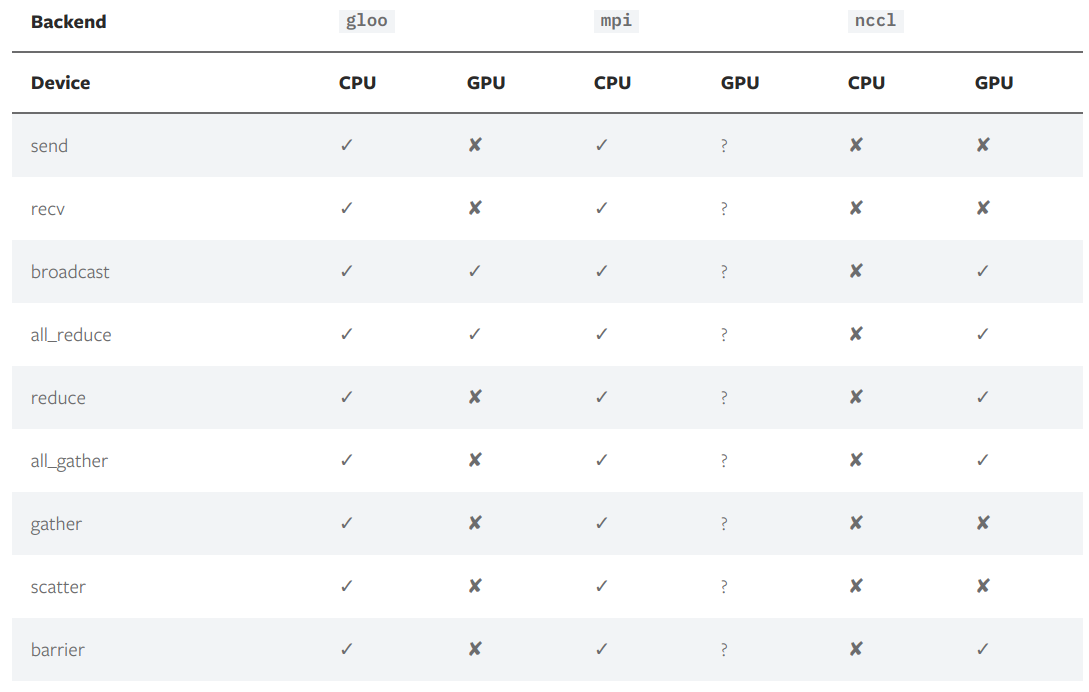
\includegraphics[width=5in,height=3in]{backends}
\caption{backends}
\end{figure}
参考:\url{https://pytorch.org/tutorials/intermediate/dist_tuto.html#our-own-ring-allreduce}
\subsection{ps vs ringAllReduce ?}
主流分布式机器学习采用的是ps架构。如tensorflow。ps全称Parameter Server Architecture 也就是参数服务器。\\
在Parameter server架构(PS架构)中,集群中的节点被分为两类:parameter server和worker。其中parameter server存放模型的参数,而worker负责计算参数的梯度。在每个迭代过程,worker从parameter sever中获得参数,然后将计算的梯度返回给parameter server,parameter server聚合从worker传回的梯度,然后更新参数,并将新的参数广播给worker。\\

pytorch 采用的是Uber Horovod的形式,也是baidu开源的ringAllReduce算法。采用PS计算模型的分布式,通常会遇到网络的问题,随着worker数量的增加,其加速比会迅速的恶化,例如resnet50这样的模型,目前的TF在10几台机器的时候,加速比已经开始恶化的不可接受了。因此,经常要上RDMA、InfiniBand等技术,并且还带来了一波网卡的升级,有些大厂直接上了100GBs的网卡,有钱任性。而Uber的Horovod,采用的RingAllReduce的计算方案,其特点是网络通信量不随着worker(GPU)的增加而增加,是一个恒定值。简单看下图理解下,GPU 集群被组织成一个逻辑环,每个GPU有一个左邻居、一个右邻居,每个GPU只从左邻居接受数据、并发送数据给右邻居。即每次梯度每个gpu只获得部分梯度更新,等一个完整的Ring完成,每个GPU都获得了完整的参数。

\section{pytorch distirbuted}
pytorch 提供distribute包。
\begin{figure}[H]
\centering
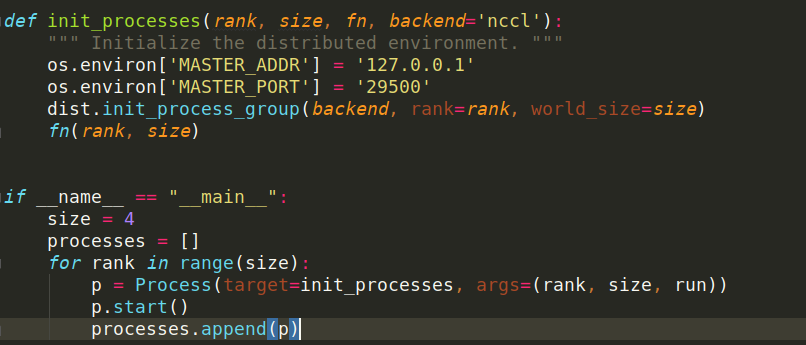
\includegraphics[width=4in,height=2in]{torch}
\caption{backends}
\end{figure}
\section{tensorflow distributed}
tensorflow 提供tf.train.ClusterSpec来创建相关cluter集群。
\begin{figure}[H]
\centering
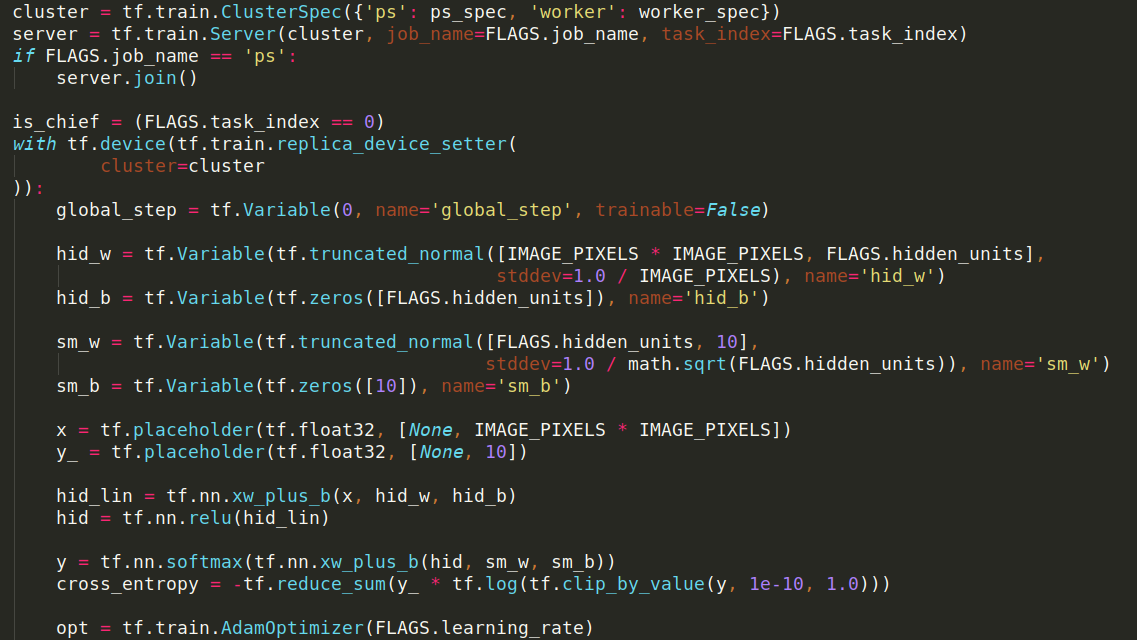
\includegraphics[width=5in,height=2.8in]{tf}
\caption{backends}
\end{figure}
分别在对应的ps,worker机器上执行相关脚本,等待所有节点加入后,训练开始
\begin{figure}[H]
\centering
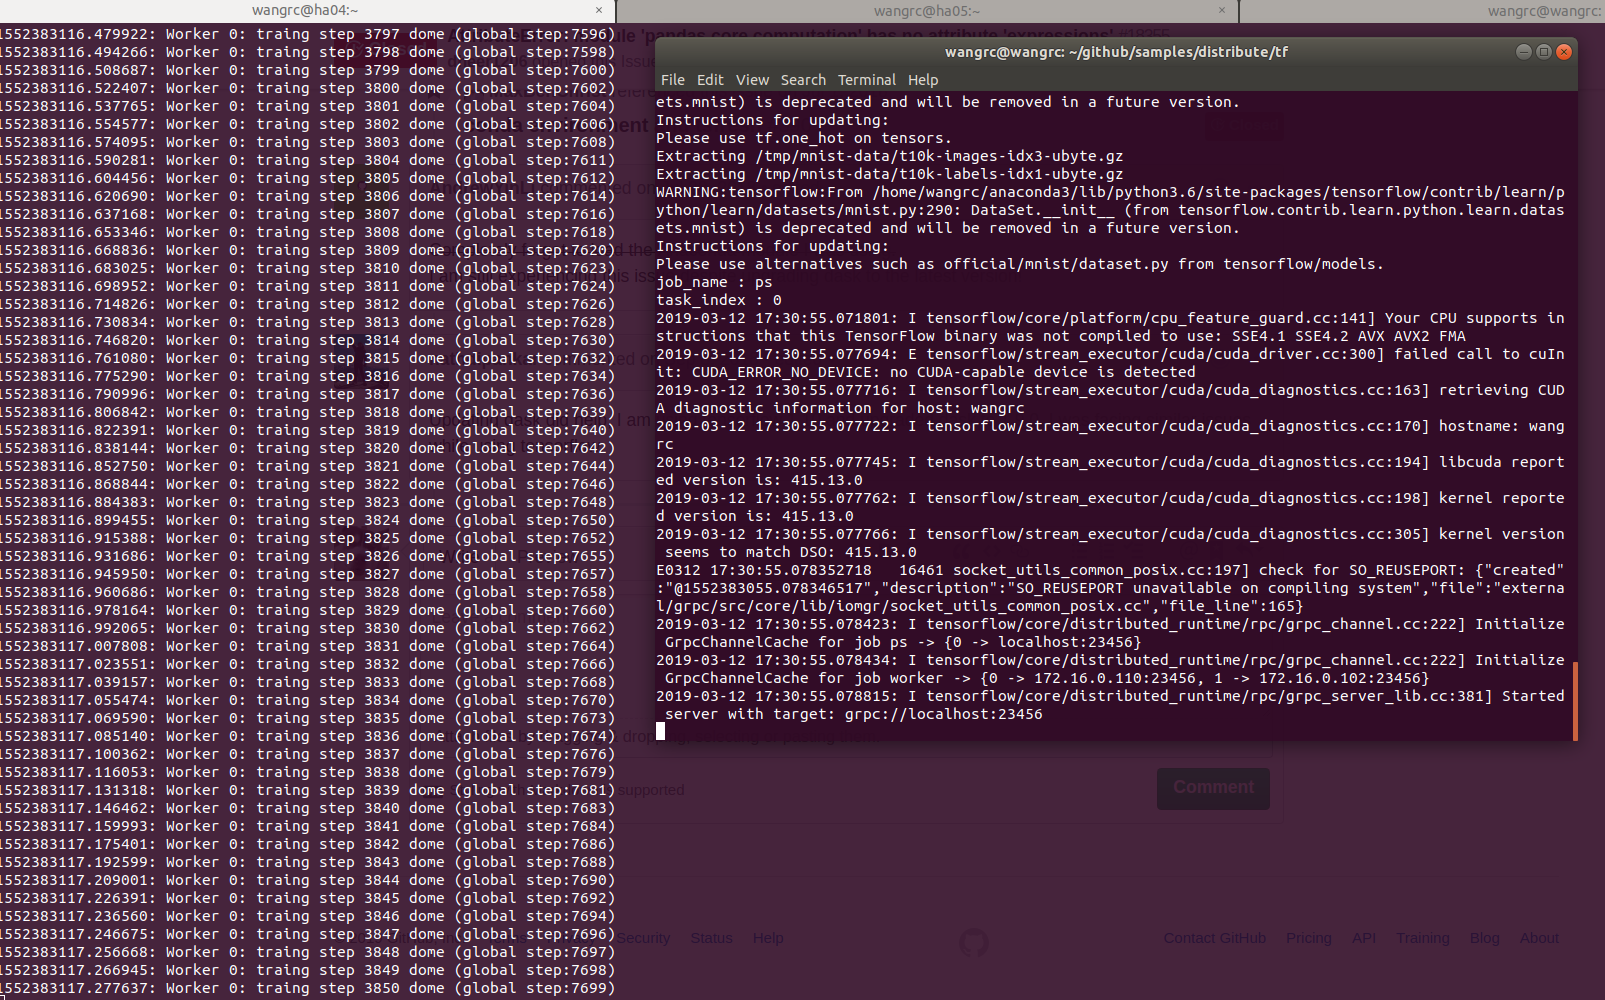
\includegraphics[width=5in,height=3in]{1}
\caption{distribute training using tensorflow gpu}
\end{figure}
\section{docker + tensorflow gpu/cpu}
\subsection{docker 是什么?}
\begin{figure}[H]
\centering
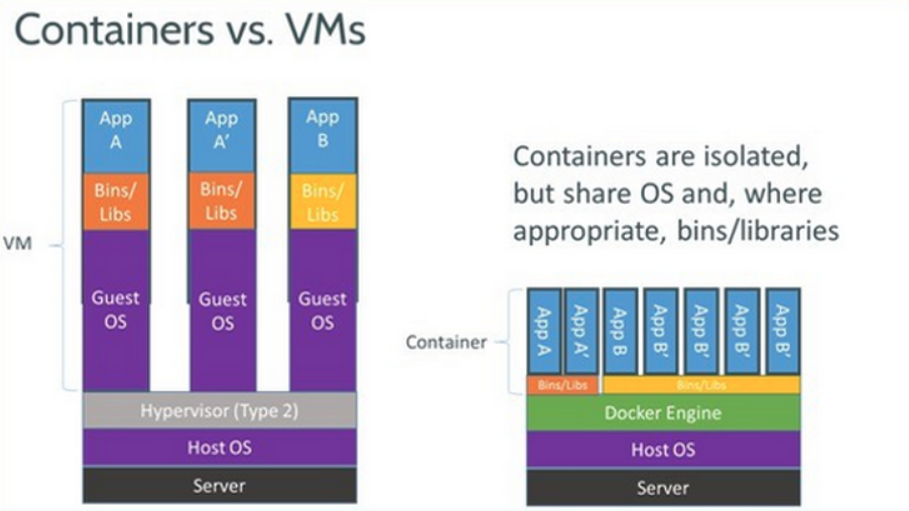
\includegraphics[width=4in,height=2in]{docker}
\caption{docker}
\end{figure}
\subsection{安装docker}
安装教程:
\url{https://docs.docker.com/install/linux/docker-ce/ubuntu/}


\noindent
\begin{itemize}
\item 查看镜像\\
docker images
\item 修改docker镜像源\\
\{ \\
"registry-mirrors": ["https://docker.mirrors.ustc.edu.cn"] \\
\}
\item 安装tensorflow docker cpu, 可以使用-tag选择想要的tf版本和python版本 \\
docker pull tensorflow/tensorflow:1.12.0-py3
\item 安装tensorflow docker gpu \\
1. 首先安装 nvidia-docker \\(https://github.com/NVIDIA/nvidia-docker)\\
2. 确认nvidia docker 安装完成\\
docker run --runtime=nvidia --rm nvidia/cuda nvidia-smi \\
\begin{figure}[H]
\centering
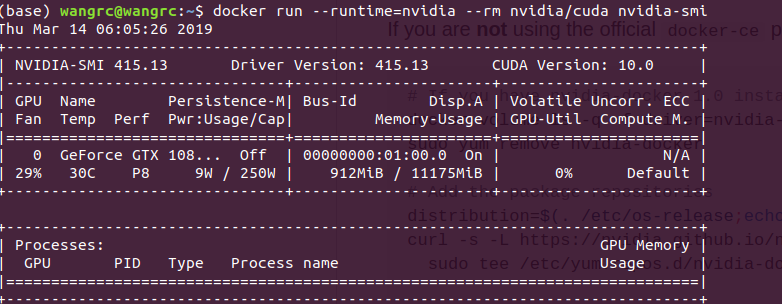
\includegraphics[width=4in,height=2in]{5}
\caption{distribute training using tensorflow gpu}
\end{figure}

3. 安装tensorflow gpu \\
docker pull tensorflow/tensorflow:1.12.0-gpu-py3\\
4. 启动支持nvidia的docker \\
docker run --runtime=nvidia -it --rm tensorflow/tensorflow:1.12.0-gpu-py3 bash\\
\begin{figure}[H]
\centering
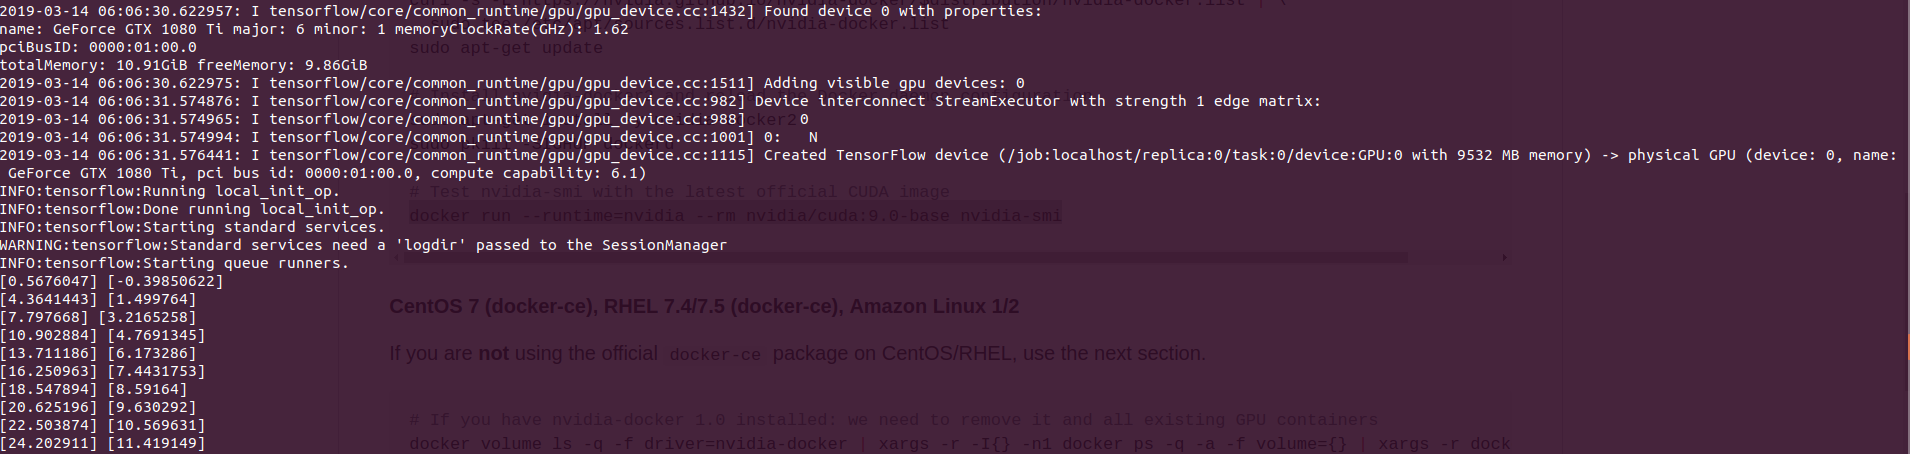
\includegraphics[width=4in,height=1.5in]{6}
\caption{training using docker tensorflow gpu}
\end{figure}
\end{itemize}

\section{k8s}
\subsection{安装k8s}
\url {https://kubernetes.io/docs/setup/}

\subsection{简介}
随着docker、容器的日渐成熟,容器编排的问题就凸显出来,大量的容器怎么去管理,怎么调度,怎么启停都成了迫切需要解决的问题。单纯地使用docker没有办法限制 cpu or gpu资源. k8s 支持为每个请求分配cpu与gpu资源. k8s优点这里就不详细列举了。
\begin{figure}[H]
\centering
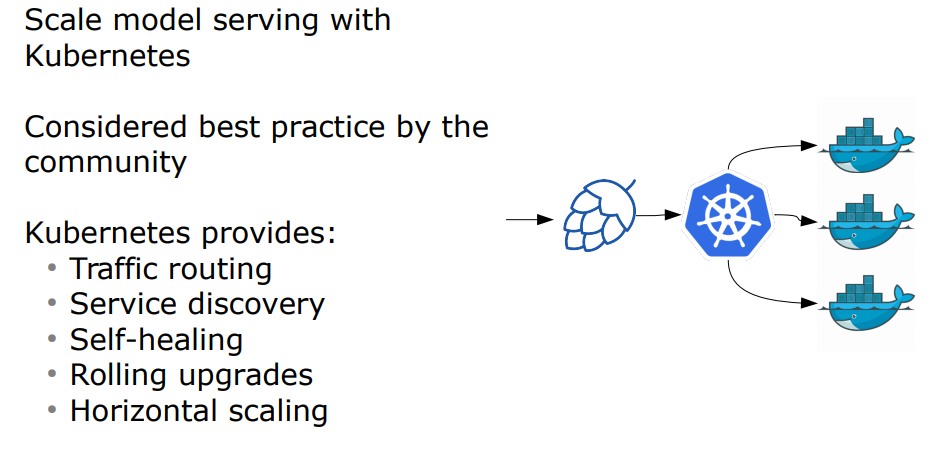
\includegraphics[width=3in,height=1.3in]{k8s}
\caption{k8s and docker}
\end{figure}

\begin{figure}[H]
\centering
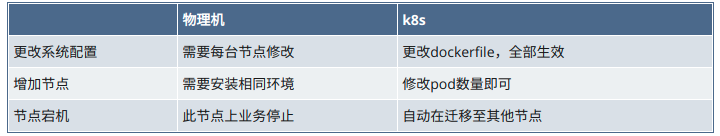
\includegraphics[width=4in,height=1in]{k8s2}
\caption{k8s 2}
\end{figure}

典型的 Kubernetes 集群包含一个 master 和很多 node。Master 是控制集群的中心,node 是提供 CPU、内存和存储资源的节点。Master 上运行着多个进程,包括面向用户的 API 服务、负责维护集群状态的 Controller Manager、负责调度任务的 Scheduler 等。每个 node 上运行着维护 node 状态并和 master 通信的 kubelet,以及实现集群网络服务的 kube-proxy。\\

Kubernetes 中部署的最小单位是 pod,而不是 Docker 容器。实时上 Kubernetes 是不依赖于 Docker 的,完全可以使用其他的容器引擎在 Kubernetes 管理的集群中替代 Docker。在与 Docker 结合使用时,一个 pod 中可以包含一个或多个 Docker 容器。但除了有紧密耦合的情况下,通常一个 pod 中只有一个容器,这样方便不同的服务各自独立地扩展。

k8s 为pod分配 gpu资源时可以指定gpu个数和类型:
\begin{figure}[H]
\centering
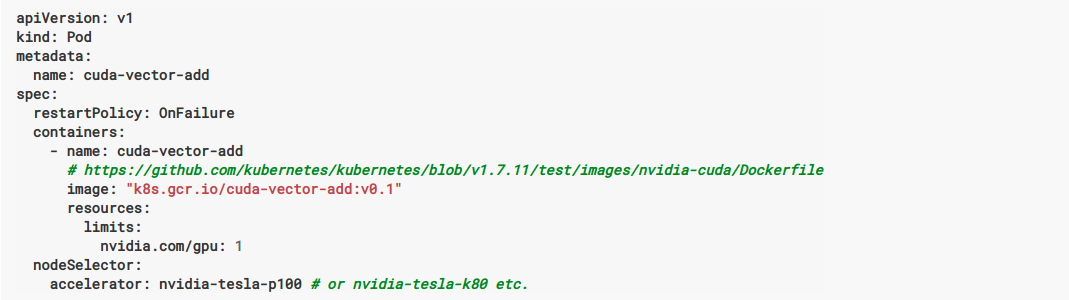
\includegraphics[width=5in,height=1.5in]{gpusc}
\caption{k8s gpu schedule}
\end{figure}
整体架构: 
\begin{figure}[H]
\centering
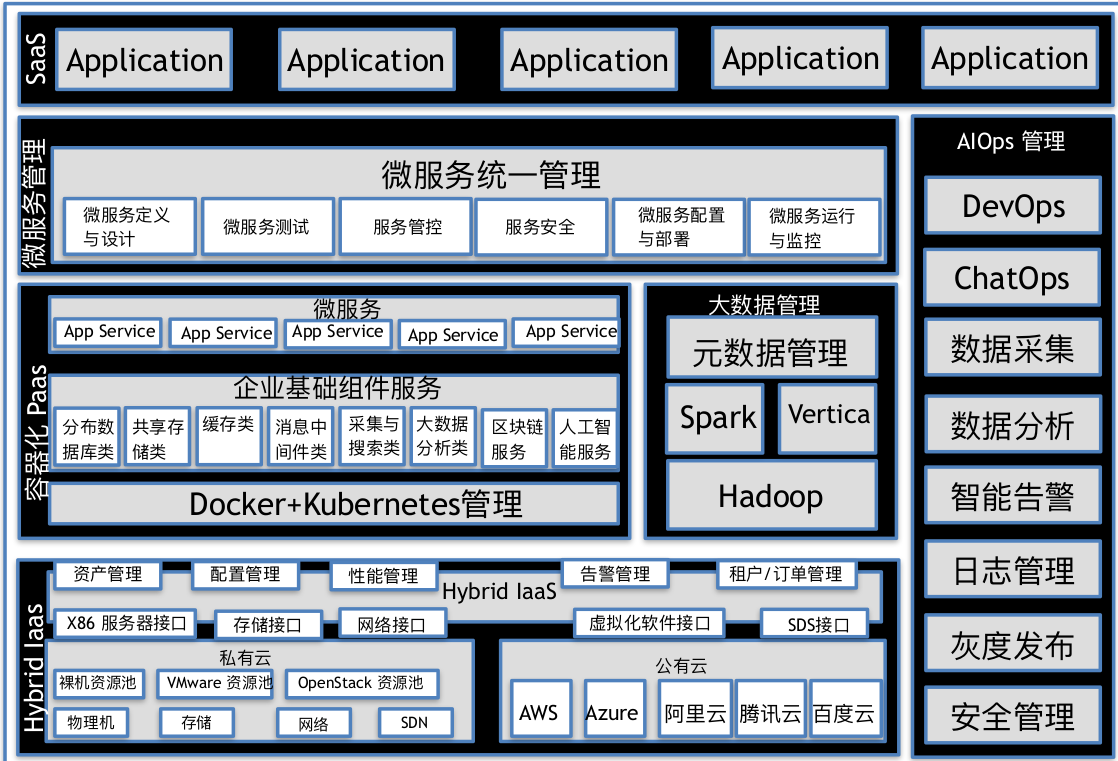
\includegraphics[width=5in,height=3.5in]{arc1}
\caption{k8s+docker 整体架构}
\end{figure}
技术构架:
\begin{figure}[H]
\centering
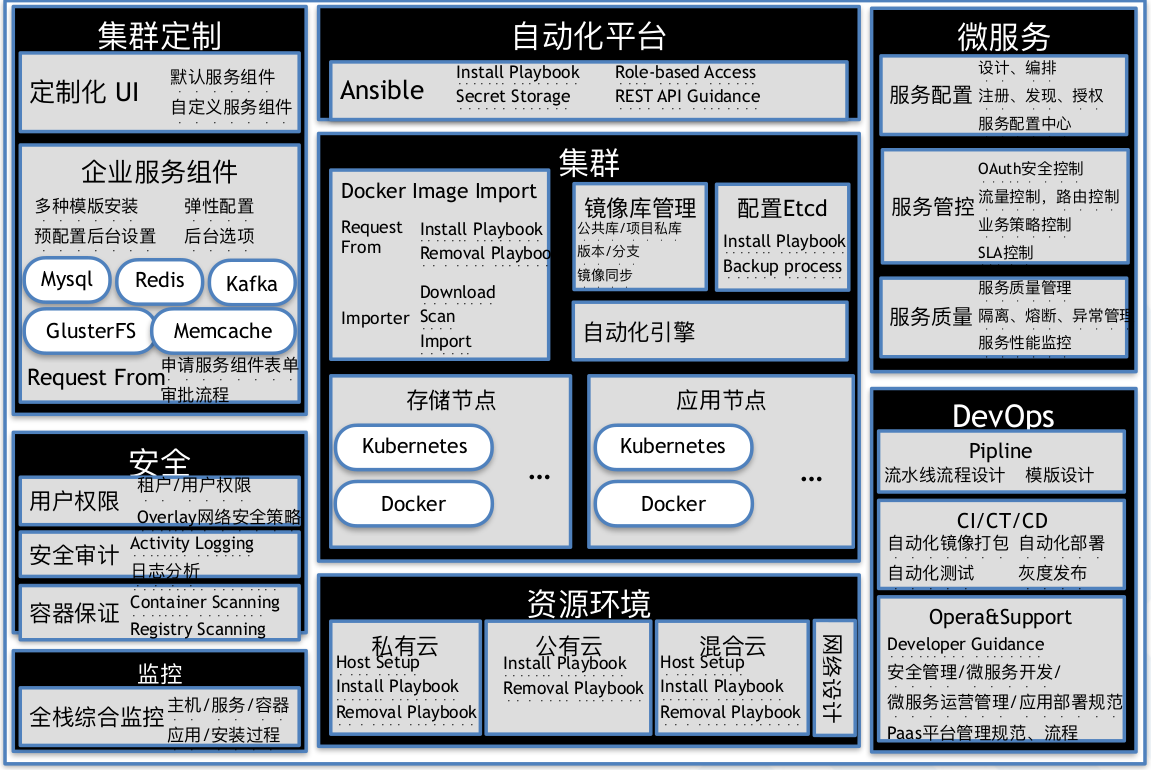
\includegraphics[width=5in,height=3.5in]{arc2}
\caption{k8s+docker 技术架构}
\end{figure}

\end{CJK*}
\end{document}




















